\setauthor{Weissengruber Nina}
\begin{figure}[!htb]
    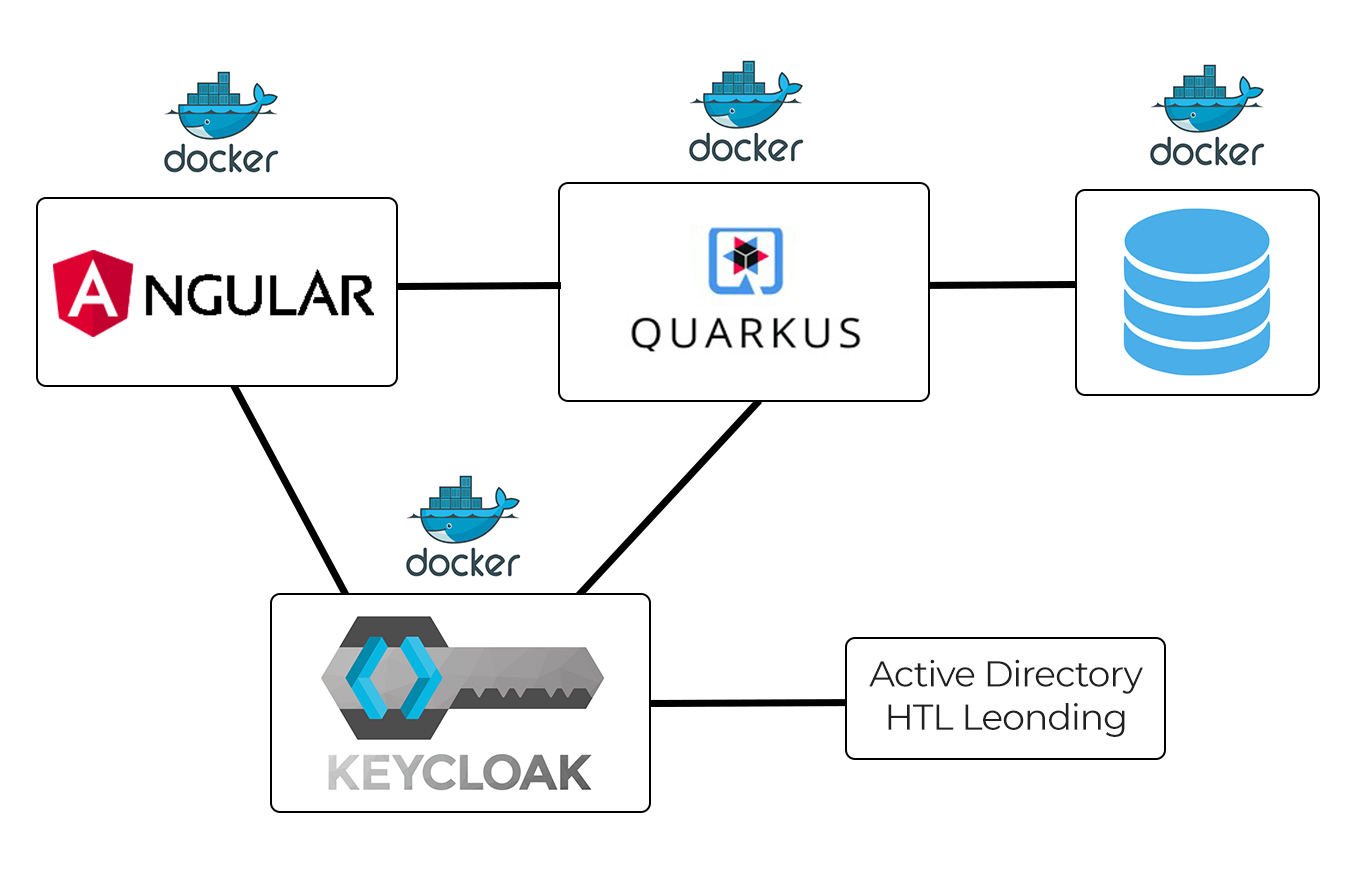
\includegraphics[width=0.5\textwidth]{pics/Systemarchitektur.png}
    \centering
    \caption{Systemarchitektur}
    \label{fig:systemarchitektur}
\end{figure}
In Abbildung \ref{fig:systemarchitektur} sieht man die Systemarchitektur.
Für diese Anwendung wurde für das Backend Quarkus verwendet, das auf eine PostgreSQL Datenbank zugreift.
Für das Frontend wurde Angular verwendet. Außerdem wurde ein Keycloak, der Zugriff auf das Active 
Directory der HTL Leonding hat und mit Frontend und Backend kommuniziert, eingebaut.

\section{Aktivitätsdiagramm}
Ein Aktivitätsdiagramm stellt eine Reihe von dynamischen Beziehungen in einem System dar.

\begin{figure}[!htb]
    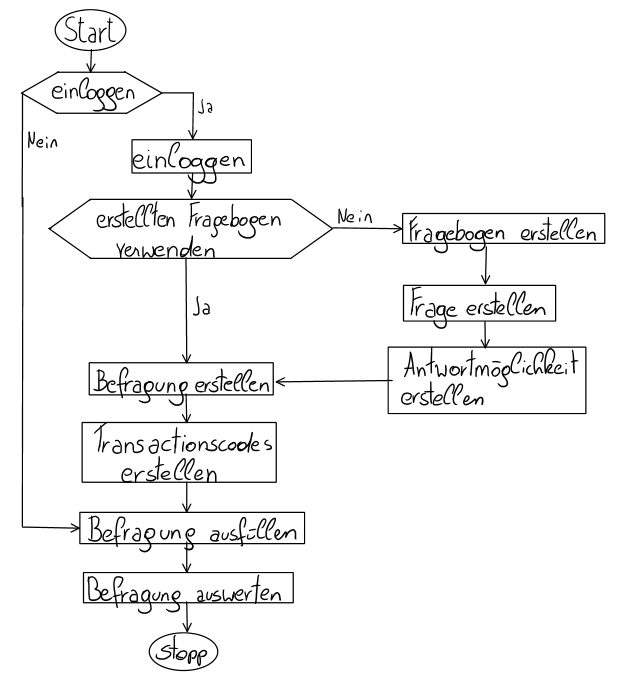
\includegraphics[width=0.5\textwidth]{pics/flussdiagramm.png}
    \centering
    \caption{Aktivitätsdiagramm}
    \label{fig:aktivitaetsdiagramm}
\end{figure}
Abbildung \ref{fig:aktivitaetsdiagramm}ist das Aktivitätsdiagramm für diese Arbeit.
Beim Start des Programms gibt es als erstes die Entscheidung, ob man sich einloggen will oder nicht. 
Möchte man sich nicht einloggen, kann man gleich die Befragung ausfüllen. Entscheidet man sich zum 
einloggen, steht man vor der Entscheidung, ob man einen bereits erstellten Fragebogen
verwenden möchte. Wenn ja, kann man eine Befragung erstellen. Möchte man keinen vorgefertigten Fragebogen 
verwenden, kann man selbst einen Fragebogen erstellen. Danach kann eine Frage erstellt und im Zuge 
dessen kann eine Antwortmöglichkeit/können Antwortmöglichkeiten erstellt werden. Danach ist es möglich, eine Befragung zu 
erstellen, um anschließend Transactions Codes zu erstellen. Danach kann man die Befragung 
ausfüllen und daraus die Befragung auswerten.

\setauthor{Raffeiner Christine}
\section{Klassendiagramm und Entity-Relationship-Modell}
\setauthor{Raffeiner Christine}
Beim Start der Arbeit wurden im Zuge der Implementierung 
ein Klassendiagramm und ein Entity-Relationship-Modell erstellt.

\subsection{Unterschied}
Bei beiden Diagrammtypen werden die Datenstrukturen und ihre Beziehungen zueinander abgebildet. 
Während jedoch Klassendiagramme dem objektorientierten Paradigma entsprechen (mit Collections, Objektidentität, usw.), 
bilden ERDs die in den Datenbanktabellen gespeicherten Datenstrukturen und deren Beziehungen ab. ERDs entsprechen dem 
relationalem Paradigma. (inkl. Erfüllung der Normalformen, des Schlüsselprinzips, usw.)
\newline
\newline
Die erste Version der Diagramme wurden mithilfe des SQL-Developers erstellt. Mehr Informationen zum SQL-Developer 
befinden sich im Kapitel \ref{chap:sqldeveloper}. \cite{noauthor_was_nodate-2}, \cite{noauthor_klassendiagramm_2022}, \cite{noauthor_klassendiagramm_nodate}

\subsection{Erste Version}
\begin{figure}[H]
    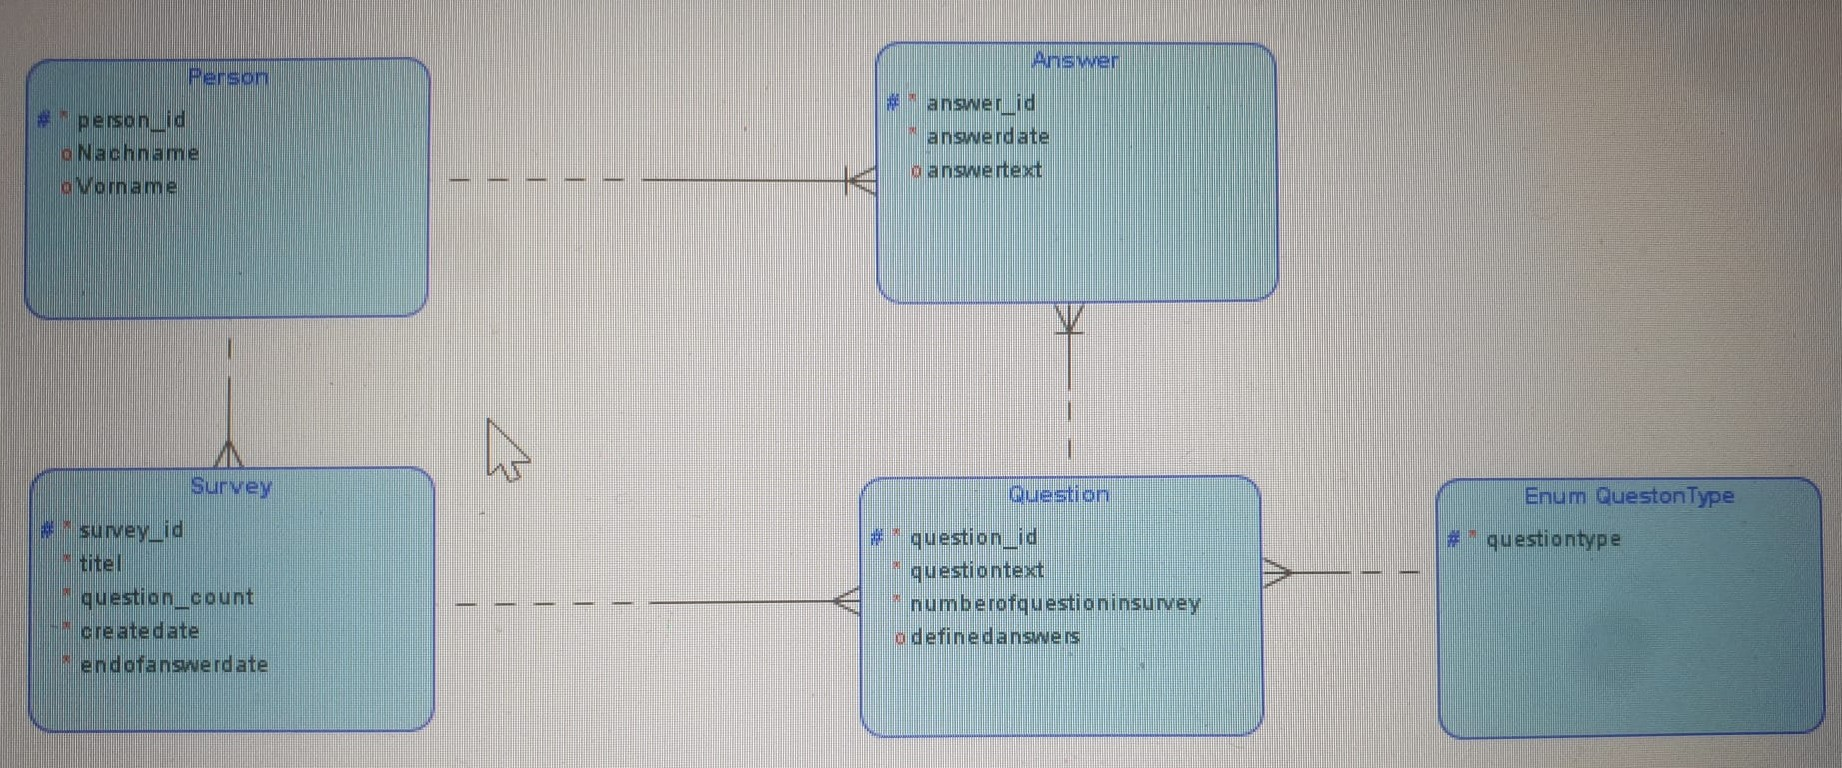
\includegraphics[width=0.8\textwidth]{pics/Datamodel_Version1.jpeg}
    \centering
    \caption{Erste Version des Datenmodelles (ERD)}
    \label{fig:cld1}
\end{figure}

\begin{figure}[H]
    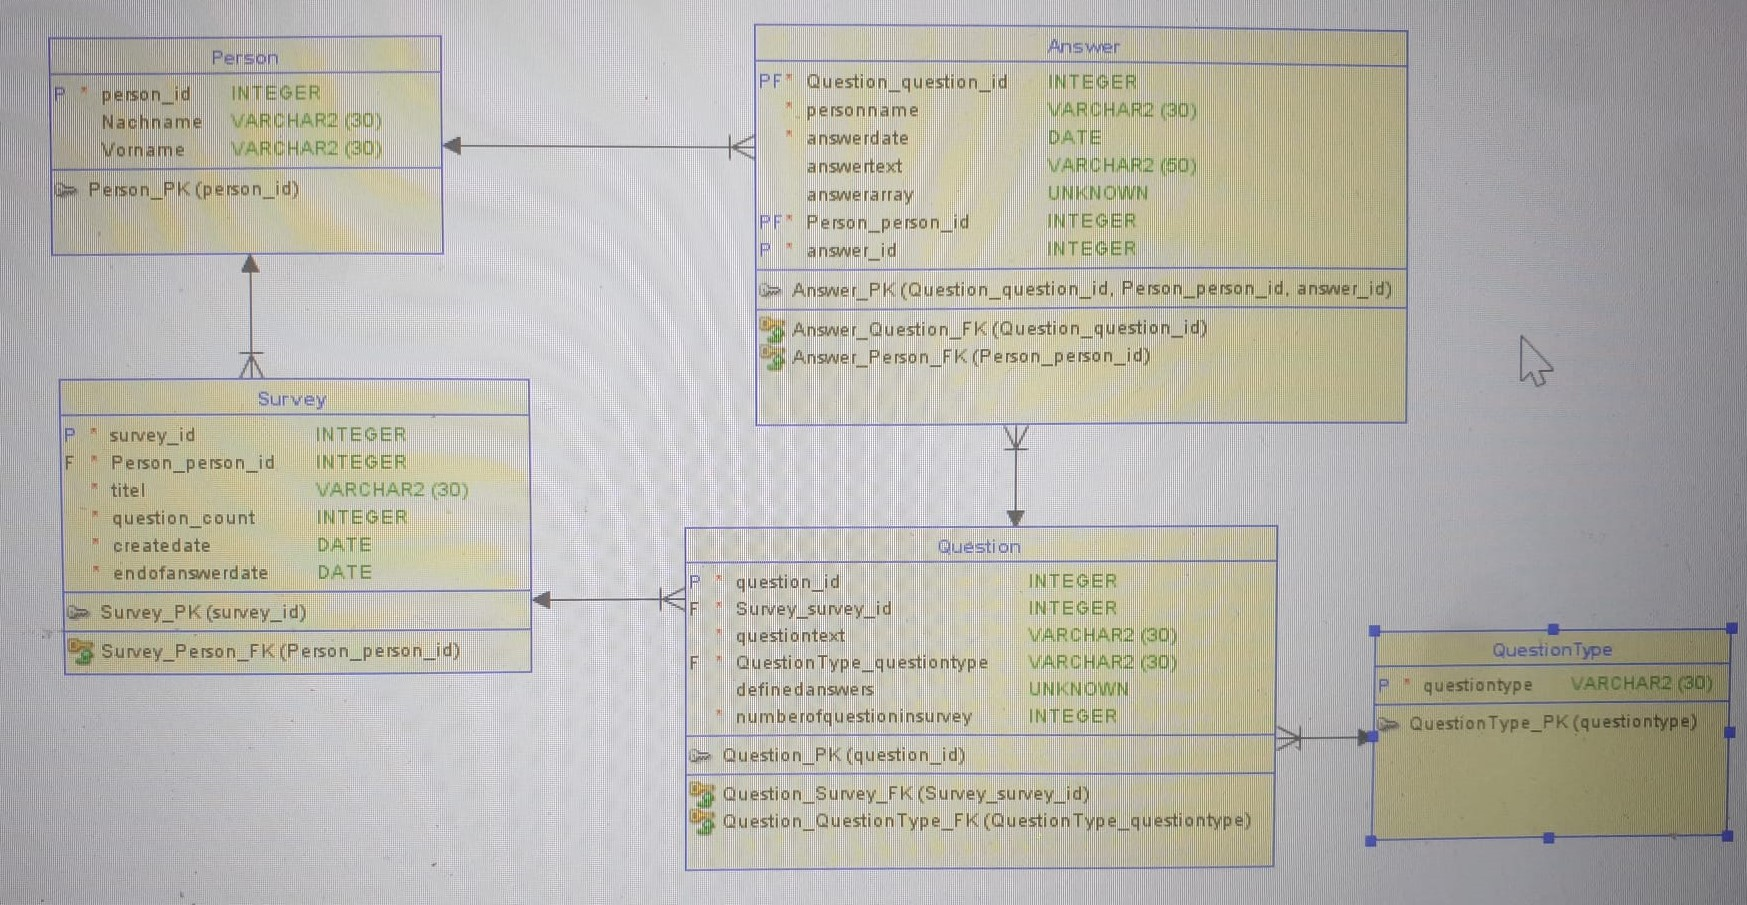
\includegraphics[width=0.8\textwidth]{pics/Datamodel_Vesion1_relational.jpeg}
    \centering
    \caption{Erste Version des Datenmodelles (CLD)}
    \label{fig:cld2}
\end{figure}
Das Datenmodell (siehe Abb. \ref{fig:cld1} und \ref{fig:cld2}) bildet eine einfache Art Fragebögen, 
zugehörige Befragungen und Antworten zu speichern, ab.
Für die leichtere Implementierung der grundlegenden Funktionen wurde in der ersten Version die Klasse Person noch zur 
Implementierung vorgesehen. Diese sollte in einer Endversion jedoch entfernt und durch die Anbindung an den Keycloak ersetzt werden.
\newline
\newline
Das Problem dieses Datenmodells bestand darin, dass nicht alle Anforderungen 
der Arbeit durch das Datenmodell abgebildet werden konnten und es auch nicht normalisiert wurde. 
\newline
Die erste Normalform wurde in dem Modell (siehe Abb. \ref{fig:cld1} und \ref{fig:cld2}) durch das Attribut definedanswers 
missachtet. Es war vorgesehen, alle möglichen Antworten in einem Attribut durch Trennzeichen abgetrennt zu speichern.
\newline
Es wurde dagegen entschieden, das Datenmodell zu überarbeiten und stattdessen ein neues Datenmodell von einem anderen Projekt als Vorlage 
zu nehmen. (siehe Kapitel \ref{chap:related_work}). 

\subsection{Normalisierung}
Unter Datenbanknormalisierung versteht man den Vorgang, Daten innerhalb einer Datenbank so effizient wie möglich zu organisieren.
Bei der Verwendung einer relationalen Datenbank kann die Normalisierung dazu beitragen, 
die Daten fehlerfrei zu halten und sicherzustellen, dass die Größe der Datenbank nicht durch 
doppelte Daten vergrößert wird. \cite{noauthor_normalisierung_2022}

\subsubsection{1. Normalform}
Die Erste Normalform (1NF) ist dann gegeben, wenn alle Informationen in einer Tabelle atomar vorliegen. \cite{noauthor_erste_nodate}

\subsection{Umstieg zu Markdown und PlantUML}
Alle weiteren Versionen des Datenmodells wurden mit PlantUML erstellt. Der Hauptgrund für den 
Wechsel bestand darin, dass die Software IntelliJ IDEA, die zum Programmieren des 
Backends verwendet wurde, diese Diagramme erstellen und anzeigen kann.
Diese können in Markdown eingebettet oder in eigenständigen Dateien mit einem Plugin gebildet werden. 
Die Teammitglieder waren mit PlantUML vertraut, was den Wechsel zusätzlich bestärkte.
\newline
\newline
Dateien mit Markdown-formatiertem Text können mit vielen Anwendungen geöffnet werden. 
Markdown-Dateien können einfach in andere Markdown-Anwendungen importieren werden.
Mehr Informationen über Markdown und PlantUML befinden sich im Kapitel \ref{chap:plantuml} und \ref{chap:markdown}.

\subsection{Zweite Version}
\begin{figure}[H]
    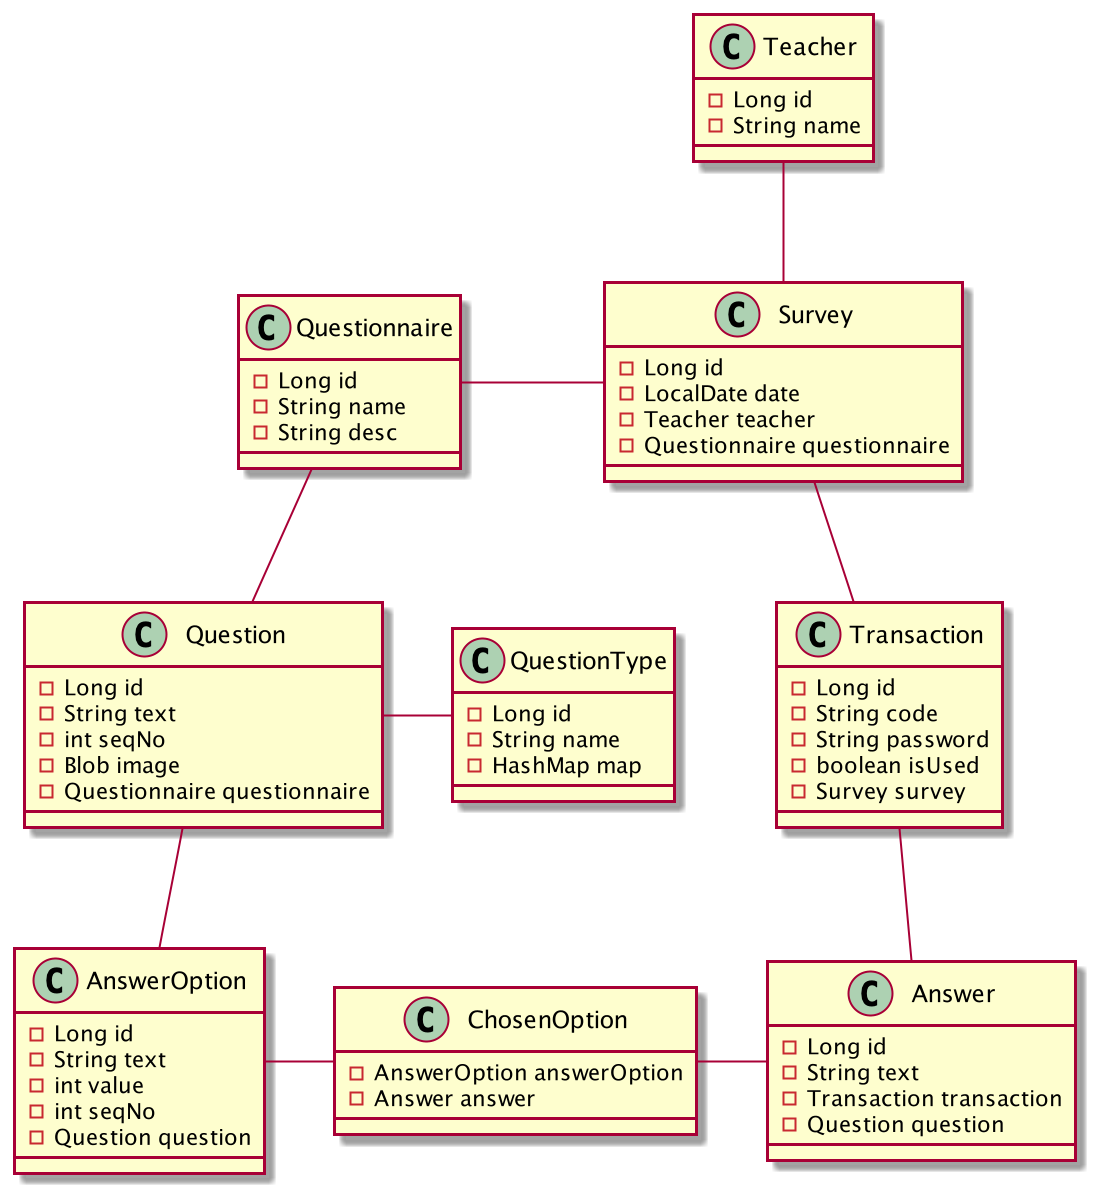
\includegraphics[width=0.8\textwidth]{pics/Datenmodel_Version2.png}
    \centering
    \caption{Zweite Version des Datenmodells}
    \label{fig:cld3}
\end{figure}
Die zweite Version des Datenmodells (siehe Abb. \ref{fig:cld3}) ist auf dem Modell eines Vorgängerprojektes aufgebaut 
(siehe Kapitel \ref{chap:related_work}). 
Erweiterungen wurden im Bereich Beantwortung der Befragung und Auswertung getätigt.
Mit den Erweiterungen konnten nun Singe-Choice, Multiple-Choice und Text-Antworten besser abgebildet werden.
Zudem wurde das Modell um die Funktion der optionalen Speicherung eines Bildes zu Fragen ergänzt.
\newline
\newline
Questionnaire stellt den Fragebogen und Survey die Befragungen dar. Es ergibt sich, dass für einen 
Fragebogen mehrere Befragungen gleichzeitig erstellt werden können.
Die Transaktionscodes stehen stellvertretend für den/die Benutzer/in und garantieren die Anonymität der Person, die den 
Fragebogen ausfüllt.

\subsection{Stabile Version}
\begin{figure}[H]
    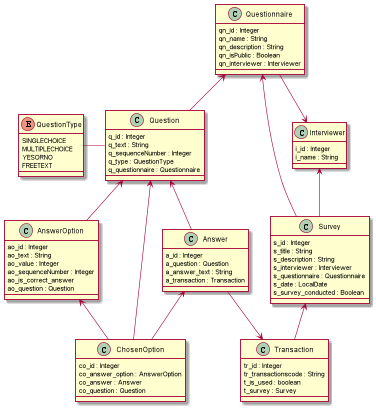
\includegraphics[width=0.8\textwidth]{pics/cld_Version3.png}
    \centering
    \caption{Zwischenversion des Datenmodells}
    \label{fig:cld4}
\end{figure}

Im Laufe der Implementierung sind weitere Änderungen am Klassendiagramm vorgenommen worden (siehe Abb. \ref{fig:cld4}), um den 
wachsenden Anforderungen gerecht zu werden. Dadurch ist beispielsweise ein zusätzliches 
Attribut im Fragebogen hinzugefügt worden (is\_public). Dieses Attribut stellt sicher, dass jede/r Benutzer/in der Applikation 
Fragebögen öffentlich zur Verfügung stellen kann. Sichtbar sind alle öffentlichen und privaten Fragebögen des Benutzers. 
\newline
Der Befragung wurde um das Attribut interviewer erweitert, um anderen Benutzern die Möglichkeit zu 
geben, öffentliche Fragebögen auszufüllen.
In der letzten signifikanten Änderung wurde das Attribut survey\_conducted hinzugefügt, 
dass besagt, ob und wie lange Personen den Fragebogen ausfüllen können. Dies dient 
dazu, den Fragebogen als Leistungsfeststellung zu verwenden.

\subsection{Endversion}
\begin{figure}[H]
    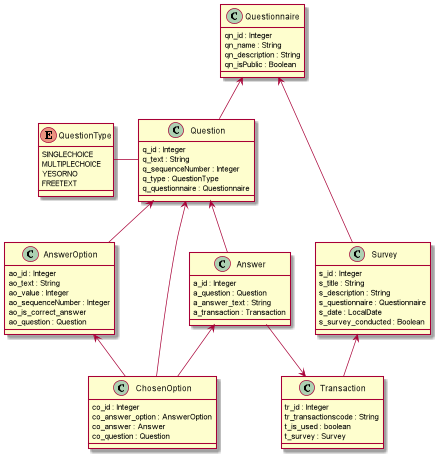
\includegraphics[width=0.8\textwidth]{pics/cld_final.png}
    \centering
    \caption{Letzte Version des Datenmodells}
    \label{fig:cld5}
\end{figure}

Mit der Implementierung des Keycloaks entfiel die Klasse Person. 
Die Speicherung der Nutzer/innen wurde durch den Keycloak übernommen. (siehe Abb. \ref{fig:cld5})
